\begin{comment}
	\pagebreak
\end{comment}

\section{Variational Auto Encoders}
\begin{comment}
	Supervised vs. Unsupervised learning: \\
	\textbf{Supervised learning:} Tries to learn a function that maps $X \Rightarrow Y$, used in classification, regression, object detection and segmentation.\\
	\textbf{Unsupervised Learning:} The Goal here is to learn the hidden structure of the data, such as in clustering, feature learning, dimensionality reduction or density estimation.\\
	\textbf{Generative Modeling (our Goal):} Given training data, learn a distribution and generate new samples drawn from the learned distribution.\\
	\begin{Figure}
 		\centering
 		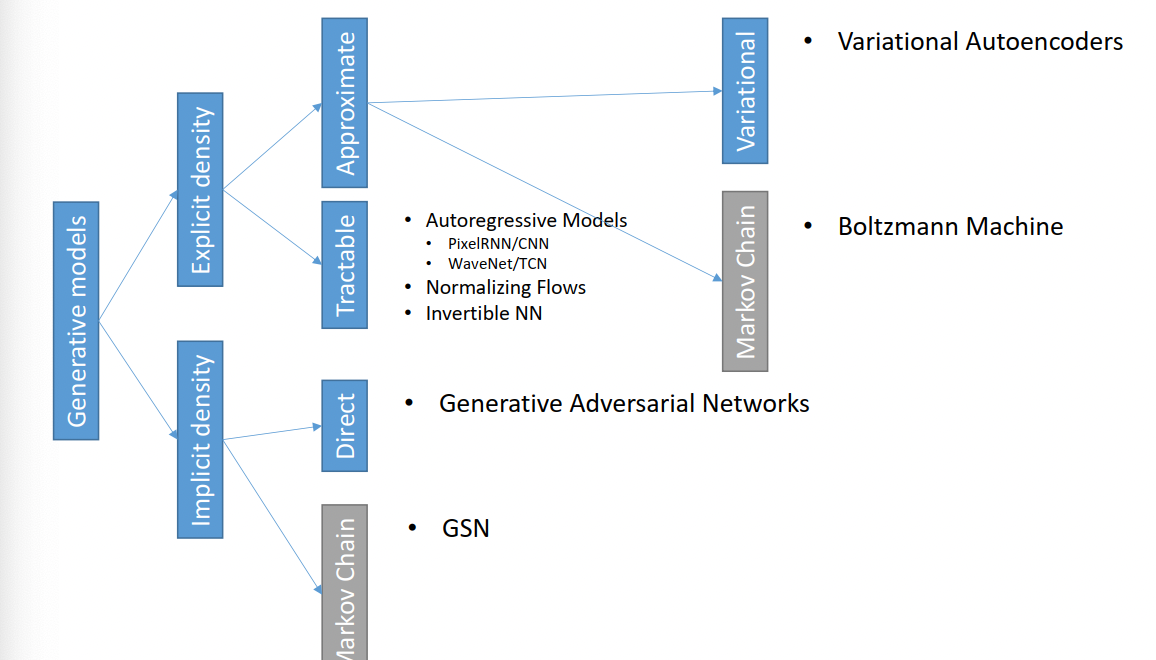
\includegraphics[width=\linewidth]{graphic/vae-taxonomy}
 		\captionof{figure}{Taxonomy of variational models}
	\end{Figure}
\end{comment}
\todo{Comment on the different models}\\

\textbf{Auto-Encoders:} optimize $\theta_f, \theta_g = \argmin \sum_n^N \norm{x_n - g(f(x_n))} ^2$\\
\begin{comment}
	The encoder projects the original input to a latent space Z. 
	The decoder samples from Z back to the input space. 
	In the optimal case, the encoder-decoder pipeline approximates the identity function of the data.\\
	
	\begin{Figure}
 		\centering
 		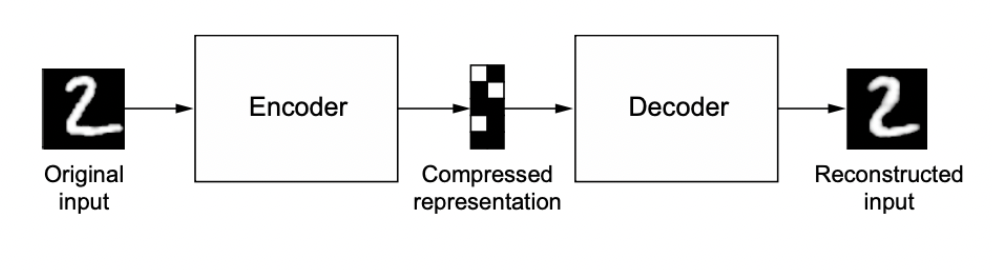
\includegraphics[width=\linewidth]{graphic/vae-ae}
 		\captionof{figure}{Auto-Encoders Model}
	\end{Figure}
	\begin{Figure}
 		\centering
 		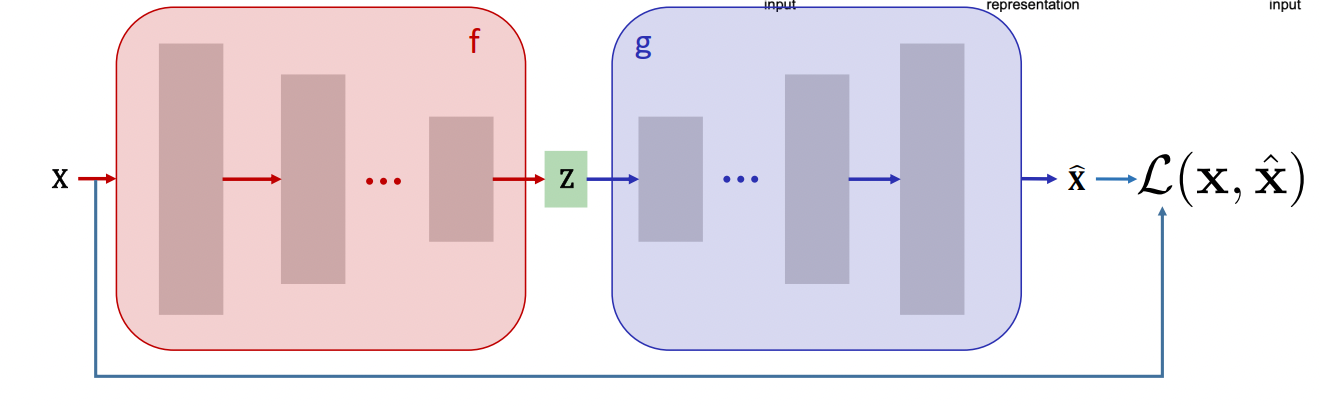
\includegraphics[width=\linewidth]{graphic/vae-ae-2}
 		\captionof{figure}{Auto-Encoders Model with loss}
	\end{Figure}
\end{comment}

\textbf{Latent Space:} find low-res meaningful DOF. Optimally the latent space is continous and interpolatable\\
\begin{comment}
	Not all dof are important, when we look at the image space (f.e. 256 x 256 x 3), we could as well sample something very random.\\
	\Note{The more dimensions the latent space has, the more information can be captured.}\\
	\textbf{Small Z (Undercomplete):} Compresses input, learns important features of input. Bad for ood samples\\
	\textbf{Big Z (Overcomplete):} Units copies input components, but hidden units might not extract meaningful structure.\\
	\begin{Figure}
 		\centering
 		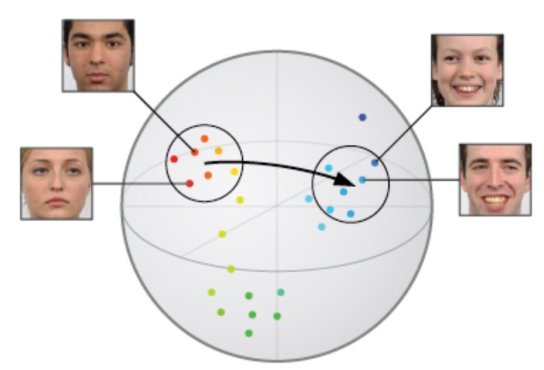
\includegraphics[width=\linewidth]{graphic/vae-latent-space}
 		\captionof{figure}{Latent space}
	\end{Figure}
\end{comment}

\textbf{PCA:} linear embedding along the principle components. This happens if f and g are linear functions.\\

\textbf{Denoising:} add gaussian noise to input, reconstruct to original\\
\begin{comment}
	\Note{The Latent space is overcomplet in this instance}\\ 
	\begin{Figure}
 		\centering
 		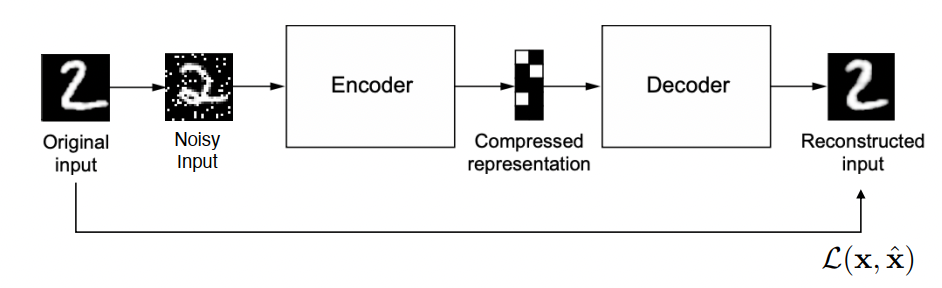
\includegraphics[width=\linewidth]{graphic/vae-denoising}
 		\captionof{figure}{VAE pipeline for denoising}
	\end{Figure}
	\begin{Figure}
 		\centering
 		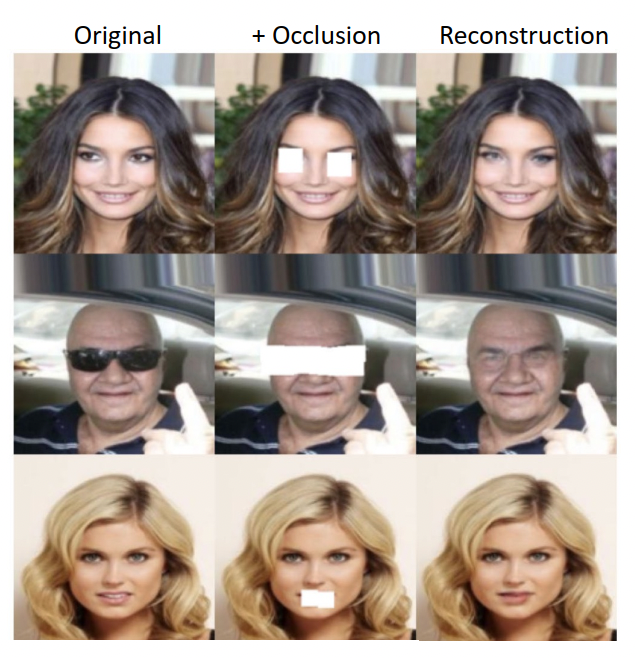
\includegraphics[width=\linewidth]{graphic/vae-denoising-ex}
 		\captionof{figure}{VAE de-noising example}
	\end{Figure}
\end{comment}

\textbf{NN:} $z = f(a(x)) = \sigma(b + Wx), \whx = g(\wha (x)) = \sigma(c + Wz)$\\

\textbf{AE limitations:} not well-structured. Training samples are easy to reconstruct, but unknown samples can not be generated.
\begin{comment}
	Variational Auto-Encoders use gaussians to model the latent space Z, the decoder can then use the distribution to sample new data.\\

	\begin{Figure}
 		\centering
 		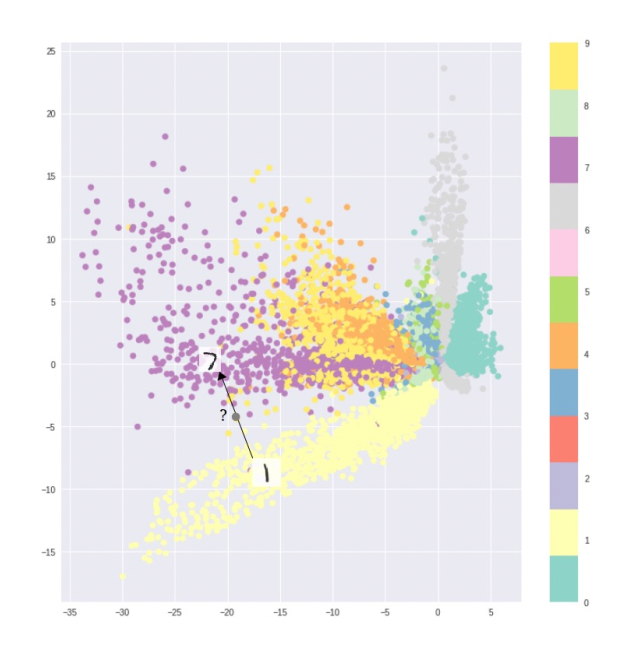
\includegraphics[width=\linewidth]{graphic/vae-mnist-embedding}
 		\captionof{figure}{AE MNIST embedding}
	\end{Figure}
\end{comment}



